%!TEX root=../GR_Schutz_light.tex
\chapter{星体的球对称解}
\label{chap10}

\section{球对称时空中的坐标}\label{sec10.1}
作为我们所研究的GR中强引力场的第一个例子,我们将讨论球对称系统。鉴于相当多的天体物理对象都近似是球形的,它们相对简单而其物理又非常重要。下面从选取能够反映这种对称性的坐标系出发。

\subsection*{球坐标系下的平直时空}
采用通常的坐标定义$(r,\theta,\phi)$,Minkowski空间的线元可以写成
\begin{equation}
\mathrm ds^2=-\mathrm dt^2+\mathrm dr^2+r^2(\mathrm d\theta^2+\sin^2\theta\,\mathrm d\phi^2).
\end{equation}
所有$r$和$t$皆为常数的曲面都是球面,精确的说,二球面——二维的球体表面。通过取$\mathrm dt=\mathrm dr=-0$可以得到球面上曲线的长度
\begin{equation}
\mathrm dl^2 = r^2(\mathrm d\theta^2+\sin^2\theta\,\mathrm d\phi^2):=r^2\,\mathrm d\Omega^2,
\label{equ10.2}
\end{equation}
其中定义了记号$\mathrm d\Omega^2$代表立体角元。我们注意到这样一个球面具有周长$2\pi r$以及面积$4\pi r^2$,即分别是$2\pi$乘上$\mathrm d\Omega^2$前系数的平方以及$4\pi$乘上$\mathrm d\Omega^2$前的系数。相对地,所有具有\eqref{equ10.2}式给出的线元形式且$r^2$独立于$\theta$和$\phi$的二曲面,都具有与二球面相同的内禀几何。

\subsection*{弯曲时空中的二球面}

\begin{figure}
\centering
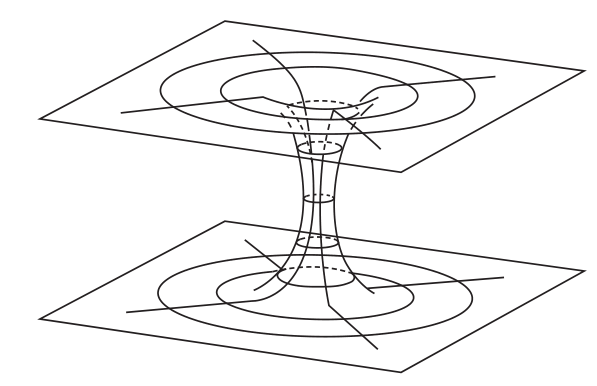
\includegraphics[width=.4\textwidth]{Pictures/fig10.1.png}
\caption{两个平面被一根环形的喉管连接起来:其具有中心(轴)对称性,但任何圆环的中心点都不在这个二平面上。}
\label{fig10.1}
\end{figure}

现在可以对于球对称时空进行更准确的描述:它意味着时空中所有位于某一个二曲面上的点都位于一个二球面上,即,其线元为
\begin{equation}
\mathrm dl^2=f(r',t)(\mathrm d\theta^2+\sin^2\theta\,\mathrm d\phi^2),
\end{equation}
其中$f(r',t)$是关于流形上另外两个坐标$r'$和$t$的未知函数。每个球面的面积都是$4\pi f(r',t)$。我们{\it 定义}球对称几何下的径向坐标满足$f(r',t):=r^2$。这代表着一个从$(r',t)$到$(r,t)$的坐标变换。任何$r$为常数且$t$为常数的曲面都是一个具有面积$4\pi r^2$以及周长$2\pi r$的二球面。由于$r$定义了球面的曲率半径以及面积,其被称为“曲率坐标”或者“面积坐标”。球心到其表面的距离与$r$之间并{\it 不存在一个先验}的关系。$r$只能描述球面自身的性质。由于其中心(在平直时空中位于$r=0$处)并不在球面上,一个球对称的空间甚至不需要在中心{\it 存在}一个点。一个简单的反例如图\ref{fig10.1}所示,那些{\it 圆环}的中心并不存在一个点。该空间包含两页通过一个“喉管”连接起来。整个相对于喉管中心轴轴对称,但轴上的点——即圆环的“中心”——并{\it 不}属于这个二维曲面。如果令$\phi$为极角,每个圆环上的线元为$r^2\,\mathrm d\phi^2$,其中$r$为用于标记每个圆环的常数。这个$r$是和我们用以描述球对称时空一类的坐标。

\subsection*{将二球面在$t$为常数的三空间中网格化}
考虑$r$和$r+\mathrm dr$处的两个球面。他们具有同样的坐标系统$(\theta,\phi)$,但至此我们并没有要求它们有什么联系。即,可以假想$r$处的球面的极点有一个取向,而$r+\mathrm dr$处的有另一个取向。明智的选择是让$\theta$和$\phi$均为常数的线与二球面{\it 正交}。根据定义,这样一条线具有一个切向量$\vec{e}_r$。鉴于向量$\vec{e}_\theta$和$\vec{e}_\phi$躺在球面上,我们要求$\vec{e}_r\cdot\vec{e}_\theta=\vec{e}_r\cdot\vec{e}_\phi=0$。这意味着$g_{r\theta}=g_{r\phi}=0$(回忆\eqref{equ3.3}式和\eqref{equ3.21}式)。这是一个因球对称而容许的坐标定义。从而度规局限于如下形式
\begin{equation}
\mathrm ds^2=g_{00}\,\mathrm dt^2+2g_{0r}\,\mathrm dr\,\mathrm dt+2g_{0\theta}\,\mathrm d\theta\,\mathrm dt+2g_{0\phi}\,\mathrm d\phi\,\mathrm dt+g_{rr}\,\mathrm dr^2+r^2\,\mathrm d\Omega^2.
\end{equation}
\subsection*{球对称时空}
由于整个时空,而不仅仅是$t$为常数的空间是球对称的,我们要求$r,\theta,\phi$均为常数的线同样也正交于二球面。否则空间中将存在一个特殊的方向。这意味着$\vec{e}_t$正交于$\vec{e}_\theta$和$\vec{e}_\phi$,或者说$g_{t\theta}=g_{t\phi}=0$。从而现在我们有
\begin{equation}
\mathrm ds^2=g_{00}\,\mathrm dt^2+2g_{0r}\,\mathrm dr\,\mathrm dt+g_{rr}\,\mathrm dr^2+r^2\,\mathrm d\Omega^2.
\end{equation}
这就是球对称时空中度规的一般形式,其中$g_{00},g_{0r}$和$g_{rr}$都是$r$和$t$的函数。我们使用了坐标自由度将其约简为最简单的形式。

\section{静态球对称时空}\label{sec10.2}
\subsection*{度规}
自然,最简单的物理情形便是一颗静止的星体或者黑洞——一个静态系统。我们{\it 定义}静态时空为这样一个时空,其时间坐标$t$满足条件:(i)所有度规分量与$t$无关;(ii)在时间反演$t\rightarrow -t$下,几何不变。第二个条件意味着在这个情形下制成的电影倒放的时候也一样。这并不能由(i)从逻辑上得到,典型的反例是一个转动的星体:时间反演改变旋转的方向,但度规却不依赖于时间。(满足条件(i)但不满足条件(ii)的时空被称为{\it 稳态}的。)

根据条件(ii)可以得到如下结论。坐标变换$(t,r,\theta,\phi)\rightarrow (-t,r,\theta,\phi)$有${\Lambda^{\bar 0}}_0=-1,{\Lambda^i}_j={\delta^i}_j$,从而
\begin{equation}
\left.\begin{array}{rcl}
g_{\bar 0\bar 0} &=& ({\Lambda^0}_{\bar 0})^2g_{00}=g_{00},\\
g_{\bar 0\bar r} &=& {\Lambda^0}_{\bar 0}{\Lambda^r}_{\bar r}g_{0r}=-g_{0r},\\
g_{\bar r\bar r} &=& ({\Lambda^r}_{\bar r})^2g_{rr}=g_{rr}.
\end{array}\right\}
\end{equation}
由于几何不变的要求(即$g_{\bar \alpha\bar\beta}=g_{\alpha\beta}$),可知$g_{0r}\equiv 0$。那么,{\it 静态}球对称时空的度规为
\begin{equation}
\mathrm ds^2=-\mathrm e^{2\Phi}\,\mathrm dt^2+\mathrm e^{2\Lambda}\,\mathrm dr^2+r^2\mathrm d\Omega^2,
\label{equ10.7}
\end{equation}
其中我们引入了$\Phi(r)$和$\Lambda(r)$用以替换两个未知的$g_{00}(r)$和$g_{rr}(r)$。在已知处处$g_{00}<0$及$g_{rr}>0$时,这个替换是容许的。稍后我们将看到这个条件对于星体内部也能保持,但对于黑洞不成立。在下一章讨论黑洞之前,我们仍然得仔细的审视一番我们的坐标系。

如果对星体这类有界系统感兴趣,我们应当有理由要求在远离星体的地方,时空几乎是平直的。这意味着可以给Einstein方程加上如下边界条件(或者说渐进正则性条件)
\begin{equation}
\lim_{r\rightarrow \infty}\Phi(r)=\lim_{r\rightarrow \infty}\Lambda(r)=0.
\end{equation}
在这个条件下我们可以说时空是{\it 渐进平直}的。

\subsection*{度规中诸项的物理诠释}
鉴于我们已经构造了能够反映时空物理对称性的坐标,度规各分量便存在着有用的物理意义。从任意半径$r_1$到半径$r_2$的本征径向距离为
\begin{equation}
l_{12}=\int_{r_1}^{r_2}\mathrm e^{\Lambda}\,\mathrm dr,
\end{equation}
假定了这是一条$\mathrm dt=\mathrm d\theta=\mathrm d\phi=0$的曲线。$g_{00}$的意义更为重要。由于度规与$t$无关,而我们从第\ref{chap7}章中得知任何沿测地线运动的粒子会有一个守恒的动量分量$p_0$,可以定义为常数$-E$:
\begin{equation}
p_0:=-E.
\end{equation}
但是一个位于时空中半径$r$处(瞬时)静止的局域{\it 惯性}观者会测量到一个不同的能量。她的四速度%
\footnote{译注:此处用词有误?}%
满足$U^i=\frac{\mathrm dx^i}{\mathrm d\tau}=0$(由于她是瞬时静止的),条件$\vec{U}\cdot\vec{U}=1$说明$U^0=\mathrm e^{-\Phi}$。那么她测量得到的能量为
\begin{equation}
E^*=-\vec{U}\cdot\vec{p}=\mathrm e^{-\Phi}E.
\end{equation}
从而我们发现一个用常数$E$标记的沿测地线运动的例子相对时空中的静态局域惯性观者具有能量$\mathrm e^{-\Phi}E$。由于在远处$\mathrm e^{-\Phi}=1$,那么可知对于一个外部的观者来说粒子在远离后的能量为$E$。我们将其称为无穷远处的能量。由于处处$\mathrm e^{-\Phi}>1$(稍后我们将看得更明白),那么对于其所经过的任何一个惯性观者来说其都有一个更大的能量。额外的能量来自于在引力场中的下落。能量问题将在\ref{sec10.9}节中的习题3中详细讨论。

这对于光子来说尤其意义重大。考虑$r_1$处发射出的一个光子,在远处被接收。如果其局域惯性系中的频率是$\nu_\text{em}$(由其发射过程决定,如光谱线),那么其局域能量便是$h\nu_\text{em}$($h$是Planck常数),守恒常数$E$为$h\nu_\text{em}\exp[\Phi(r_1)]$。当被远处的观者测量到时,其具有能量$E$,那么频率$E/h=\nu_\text{rec}=\nu_\text{em}$。光子的{\it 红移}定义为
\begin{equation}
z=\frac{\lambda_\text{rec}-\lambda_\text{em}}{\lambda_\text{em}}=\frac{\nu_\text{em}}{\nu_\text{rec}}-1,
\end{equation}
从而
\begin{equation}%box required
z=\mathrm e^{-\Phi(r_1)}-1.
\end{equation}
这个重要的式子触及了$\mathrm e^\Phi$的物理意义。(与第\ref{chap2}章中的计算相对比。)

\subsection*{Einstein张量}
可以证明,对于形如\eqref{equ10.7}式的度规,Einstein张量有分量
\begin{align}
G_{00}&=\frac{1}{r^2}\mathrm e^{2\Phi}\frac{\mathrm d}{\mathrm dr}[r(1-\mathrm e^{-2\Lambda})],\\
G_{rr}&=-\frac{1}{r^2}\mathrm e^{2\Lambda}(1-\mathrm e^{-2\Lambda})+\frac{2}{r}\Phi',\\
G_{\theta\theta}&=r^2\mathrm e^{-2\Lambda}[\Phi''+(\Phi')^2+\Phi'/r-\Phi'/\Lambda'-\Lambda'/r],\\
G_{\phi\phi}&=\sin^2\theta G_{\theta\theta},
\end{align}
其中$\Phi':=\mathrm d\Phi/\mathrm dr$。其他全部分量都为零。

\section{静态理想流体的Einstein方程}\label{sec10.2}
\subsection*{应力-能量张量}
我们对静态星体感兴趣,即没有运动的流体。$\vec{U}$仅有的非零分量为$U^0$。此外,归一化条件
\begin{equation}
\vec{U}\cdot\vec{U}=-1
\end{equation}
给出,如我们之前所看到的那样
\begin{equation}
U^0=\mathrm e^{-\Phi},\quad U_0=-\mathrm e^{\Phi}.
\end{equation}
那么由\eqref{equ4.38}式,可以给出$\mathbf T$的分量:
\begin{align}
T_{00}&=\rho\mathrm e^{2\Phi},\\
T_{rr}&=p\mathrm e^{2\Lambda},\\
T_{\theta\theta}&=r^2p,\\
T_{\phi\phi}&=\sin^2\theta T_{\theta\theta}.
\end{align}
其他全部分量为零。
\subsection*{状态方程}
应力-能量张量包含了$p$和$\rho$,但它们可能由一个状态方程相联系。对于处于局域热平衡态的简单流体,总存在着如下形式的关系
\begin{equation}
p=p(\rho,S),
\end{equation}
给出了压强$p$对于能量密度$\rho$和比熵$S$的关系。我们经常处理那些熵可以被看做是常数的情形(具体而言,改变量小到可以忽略),那么就有关系
\begin{equation}
p=p(\rho).
\end{equation}
这个关系对于不同的流体自然有不同的函数形式。我们将假定{\it 某些}这类关系始终存在。
\subsection*{运动方程}
守恒律(\eqref{equ7.6}式):
\begin{equation}
T^{\alpha\beta}_{;\beta}=0.
\end{equation}
自由指标的每一个取值都包含了一个方程。由于对称性,其中只有一个式子不会恒为零:$\alpha=r$的情形。即
\begin{equation}
(\rho+p)\frac{\mathrm d\Phi}{\mathrm dr}=-\frac{\mathrm dp}{\mathrm dr}.
\end{equation}
这个式子告诉我们为使流体在引力场中静止所需要的压强梯度,这个效应依赖于$\mathrm d\Phi/\mathrm dr$。
\subsection*{Einstein方程}